% Introduction
\section{Introduction}

%Paper Flow

%Since a large-scale is hard to implement, we make simulation instead.

%P1: Background  
Information and Communication Technology (ICT) equipment \cite{zeadally2012energy} has exploded 
on the scene in the last twenty years, leading to an obvious ascent of Internet-of-Things \cite{atzori2010internet},
such as wireless sensor networks[], mobile campus networks[], mobile gaming community, etc.


%P2: Problem
%NB problem and a brief introduction of the existing works
Neighbor discovery is a fundamental step of constructing a wireless network, based on 
which the network can implement further applications such as routing and broadcasting.
The core aim is for each node in the network to discover the nodes in its sensing range 
with one-hop communication. A number of existing works \cite{dutta2008practical,kandhalu2010u,
bakht2012searchlight,sun2014hello,chen2015heterogeneous,
wang2015blinddate,qiu2016talk,mcglynn2001birthday,
vasudevan2009neighbor,you2011aloha,song2014probabilistic} have been proposed 
to deal with this issue, some of which are based on deterministic techniques while others
are probabilistic methods.


%P3 and P4: motivation & crucial challenges
%key word: large-scale network partially-connected network
%point out problem issue
Unfortunately, the network model adopted in the current researches is disengagement from the reality networks.
While the deterministic approaches is efficient to discovery the neighbor
for two nodes, there exists some crucial problems when transferred to multiple node scenario.
Some methods can not solve the collision issue when more than one neighbors are transmitting simultaneously. 
Others follows a simple protocol that each node send a beacon at both beginning and end of an active slot, 
which is assumed only costing little time compared to a complete time slot in two node scenario. Nevertheless,
a node needs to sends a package containing all its information in a complete time slot in multiple node scenario,
otherwise the neighbor can not identify which neighbor the received beacon belongs to.
Relatively, the probabilistic approach can well deal with multiple node scenario but only consider
the network is fully-connected, the topology of which is a complete graph. 
Deploying a fully-connected network in a large-scale area is technically impractical 
due to the limited sensing range of devices communication.
How far the other nodes can be detected as a neighbor for a mobile equipment  
depends on criterion such as the received signal strength.

To our best knowledge, no relevant researches have focused on a more 
practical scenario in a large-scale network, where nodes are partially-connected
with each other. In other words, a node can only discover a fraction of nodes of the
total network in its limited radio sensing range, which can be called its neighbors.





 
 
 %P4 distribution
 In this paper, we consider the neighbor discovery process in a larger-scale networks,
 where the nodes are partially-connected. To put it more practical, 
 we take the distribution of the nodes in the network into consideration.
 As fully studied in \cite{wang2013gaussian} , the nodes in wireless sensor networks are likely to 
 follow a uniform or a Gaussian distribution as showed in Fig. \ref{distribution}, according to the specific applications of the networks.
 The crucial result is that the distribution of sensor deployment consequently plays a vital role in 
 determining the intrusion detection capability of a sensor node.

Based on this, we propose Alano\footnote{Alano is the god of luck in Greek mythology }, 
a nearly optimal probability based algorithm for sensor nodes to discover neighbors 
in a partially-connected wireless sensor network.
 
 \begin{figure}[!t]
\centering
\subfigure[uniform distribution]{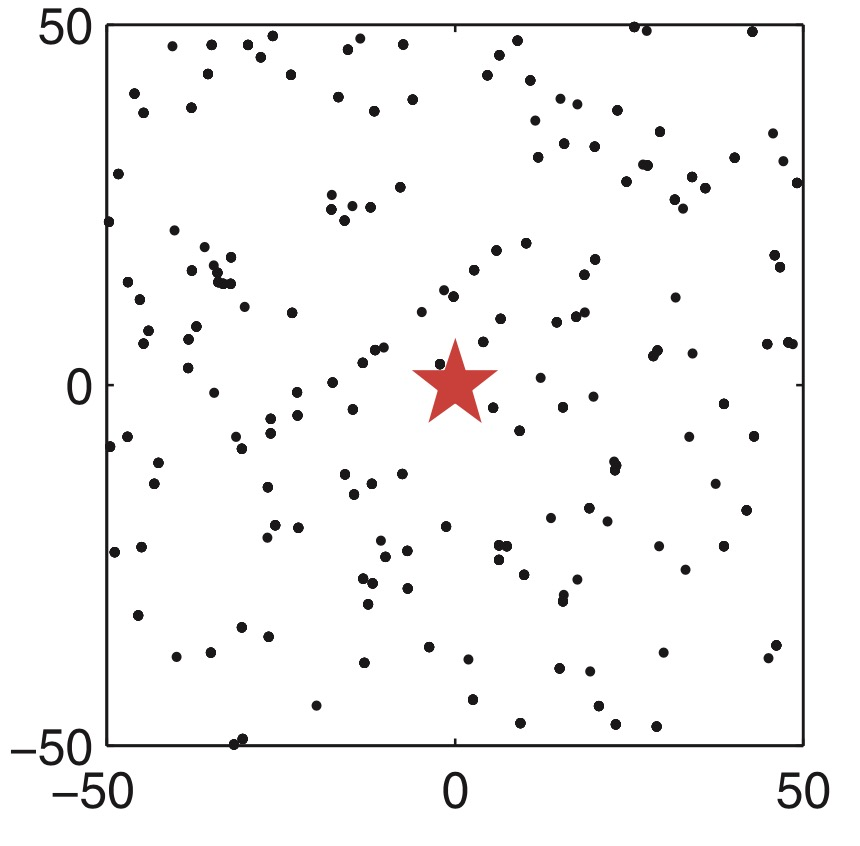
\includegraphics[width=1.7in]{./Figure/uniform.jpg}}
\vspace{0.03in}
\subfigure[Gaussian distribution]{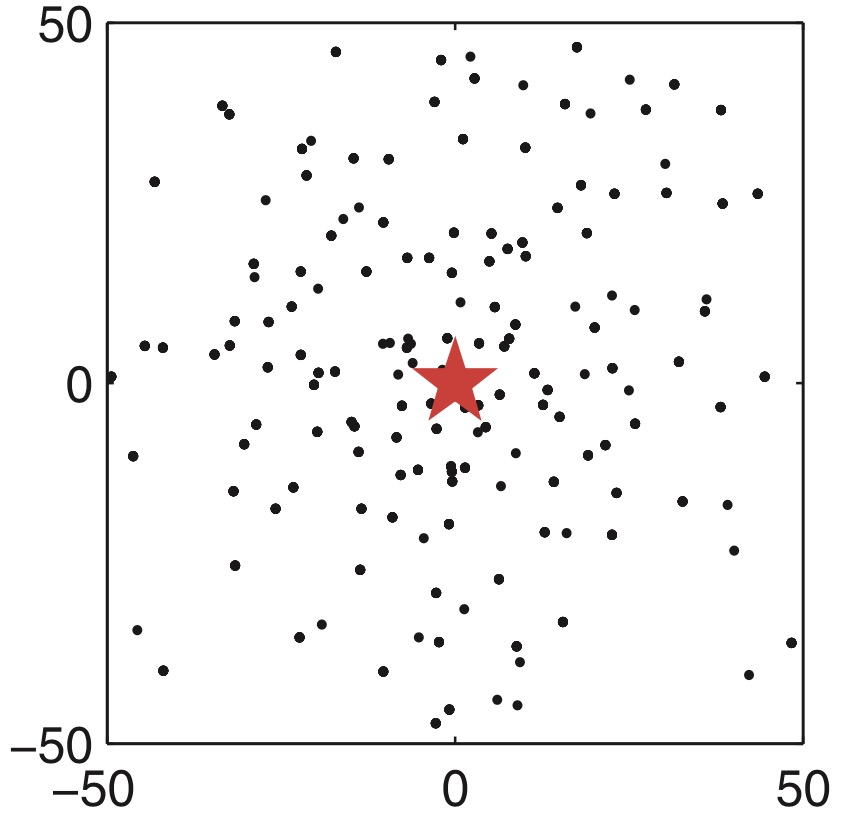
\includegraphics[width=1.7in]{./Figure/normal.jpg}}
\caption{WSN deployments following uniform and Gaussian distribution.}
\label{distribution}
%\vspace{-0.2in}
\end{figure}


 
%P5 energy-efficient network
 

Among the partially-connected networks, there is a special 
one named energy-efficient network.
Wireless sensor network is a typical energy-efficient network that all the sensor nodes have to maintain 
strict power budgets to attain years of lifetime\cite{dunkels2011contikimac}.
Duty cycle, a widely used mechanism to   , is utilized to power-awareness ought to be fully taken into consideration.
Correspondingly, the neighbor discovery process needs adjustment to deal with the dilemma between 
a balance of energy-efficiency and low-latency.

%P5 why and how we can
% treat the partially-connected scenario carefully and model the nodes distribution
%we make analysis and calculate the optimal probability based on the specific distribution.
%we utilized the initiative concept of deterministic approaches to 
%to align the wake-up time slot of the neighbors and guarantee a bound.



%P6 Brief Evaluation Analysis 
%the simulation data to support && highlight our work

%P7 Contribution
%Model the distribution of nodes
%for the global duty cycle scenario
%for the local duty cycle scenario

In this paper, we first focus on the mathematical analysis of the distribution of the nodes in the networks.
We give an expectation of neighbor number for each node in a network which obey****
propose Alano\footnote{Alano is the god of luck in Greek mythology }, 
a RDS-Alano algorithm for partially-connected networks 
as well as a TP-Alano algorithm for the energy-effienct networks.
The main contributions of this paper are summarized as follows:
%In this paper, we propose a new method to construct sequence
%we propose improved algorithms for both scenarios and our contributions are as follows:
\begin{itemize}
\item[1)] We model the distribution of nodes in their networks and analyse the 
expectation number of neighbors of a node in uniform distribution and normal
distribution and then propose Alano, a strategy
\item[2)] We propose a Relaxed DifferenceSet based Alano algorithm (RDS-Alano) 
for the global duty cycle scenario. 
\item[3)] We propose a Traversing Pointer based Alano algorithm (TP-Alano) 
for the local duty cycle scenario. 
\end{itemize}



%P8 Remaining structure

The remainder of the paper is organized as follows.
The next section highlights some related work and 
puts forward some serious problems. 
Some notion definitions and the system model are given in Section
\ref{sectionmodel}. 
We analyse the node's expectation number of neighbors and 
propose Alano algorithm in \ref{PCN} as a foundation.
Section \ref{EEN} describes the RDS-Alano algorithm for global
duty cycle scenario and TP-Alano algorithm for local duty cycle scenario
respectively in energy-efficient networks.
We have conducted extensive simulations, and the results are shown in Section
\ref{Evaluation}. Finally, we conclude the paper in Section
\ref{Conclusion}.


